\documentclass[11pt, openany, a4paper]{article}

\usepackage{etex}
\usepackage{fullpage}
\usepackage{pstricks,pstricks-add,pst-math,pst-xkey}
\usepackage[frenchb]{babel}
%\usepackage{slashbox}
\usepackage{graphicx}
\usepackage{amsmath,amssymb,amstext,amsthm}
%\usepackage{comment}
\usepackage[utf8]{inputenc}
\usepackage[OT1]{fontenc}
\usepackage{pgf,tikz}
\usepackage{pgfplots}
\usepackage{floatpag}
\usepgfmodule{shapes}
\usetikzlibrary{arrows,patterns}
\usepackage{floatflt}
\usepackage{import}
\usepackage{xcolor}
\usepackage{natbib}
%\usepackage{fourier-orns}

\newcounter{moncompteur}
\newtheorem{q}[moncompteur]{ \textbf{Question}}{}
\newtheorem{prop}[moncompteur]{ \textbf{Proposition}}{}
\newtheorem{df}[moncompteur]{ \textbf{Définition}}{}
\newtheorem*{df*}{ \textbf{Définition}}{}
\newtheorem{rem}[moncompteur]{ \textbf{Remarque}}{}
\newtheorem{theo}[moncompteur]{ \textbf{Théorème}}{}
\newtheorem{conj}[moncompteur]{ \textbf{Conjecture}}{}
\newtheorem{cor}[moncompteur]{ \textbf{Corollaire}}{}
\newtheorem{lm}[moncompteur]{ \textbf{Lemme}}{}
%\newtheorem{nota}[moncompteur]{ \textbf{Notation}}{}
%\newtheorem{conv}[moncompteur]{ \textbf{Convention}}{}
\newtheorem{exa}[moncompteur]{ \textbf{Exemple}}{}
\newtheorem{ex}[moncompteur]{ \textbf{Exercice}}{}
%\newtheorem{app}[moncompteur]{ \textbf{Application}}{}
%\newtheorem{prog}[moncompteur]{ \textbf{Algorithme}}{}
%\newtheorem{hyp}[moncompteur]{ \textbf{Hypothèse}}{}
\newenvironment{dem}{\noindent\textbf{Preuve}\\}{\flushright$\blacksquare$\\}
\newcommand{\cg }{[\kern-0.15em [}
\newcommand{\cd}{]\kern-0.15em]}
\newcommand{\R}{\mathbb{R}}
\newcommand{\K}{\mathbb{K}}
\newcommand{\N}{\mathbb{N}}
\newcommand{\Z}{\mathbb{Z}}
\newcommand{\C}{\mathbb{C}}
\newcommand{\U}{\mathbb{U}}
\newcommand{\Q}{\mathbb{Q}}
\newcommand{\B}{\mathbb{B}}
\newcommand{\card}{\mathrm{card}}
\newcommand{\norm}[1]{\left\lVert#1\right\rVert}
\pgfplotsset{compat=newest}
\newcommand{\La}{\mathcal{L}}
\newcommand{\Ne}{\mathcal{N}}
\newcommand{\D}{\mathcal{D}}
\newcommand{\Ss}{\textsc{safestay}}
\newcommand{\Sg}{\textsc{safego}}
\newcommand{\M}{\textsc{move}}
\newcommand{\E}{\mathcal{E}}
\newcommand{\V}{\mathcal V}
\setlength{\parindent}{0pt}
\newcommand{\myrightleftarrows}[1]{\mathrel{\substack{\xrightarrow{#1} \\[-.6ex] \xleftarrow{#1}}}}
\newcommand{\longrightleftarrows}{\myrightleftarrows{\rule{1cm}{0cm}}}

\definecolor{bleuclair}{rgb}{0.75,0.75,1.0}
\newcommand{\ANNOT}[1]{
  ~\linebreak
  \centerline{
    %{\Huge{\danger}}
    \large\fcolorbox{black}{bleuclair}{
      \begin{minipage}[h]{.8\linewidth}
      #1
      \end{minipage}
    }
    %{\Huge{\danger}}
  }
}

\newcommand\tikzmark[1]{%
  \tikz[overlay,remember picture,baseline] 
  \node[anchor=base](#1){};}

\newcommand\MyLine[3][]{%
  \begin{tikzpicture}[overlay,remember picture]
    \draw[#1] (#2.north west) -- (#3.south east);
  \end{tikzpicture}}


\graphicspath{{.}}
\newcommand{\e}[1]{$\times 10^{#1}$}
\begin{document}

\section*{Introduction}

Définition : collaborative filtering

Position du problème : 
Attentes vis-à-vis des algorithmes (précision/temps de réponse/ajout rapide d'un rating/cold start...)

Efficacité peut varier selon la forme du jeu de données (sparsity...)

Objectif : Implémenter (en Matlab) et comparer différents algorithmes en terme de précision et de temps d'exécution sur différents jeux de données, mettre en relief les compromis à faire.

\section{Les algorithmes utilisés}
	\subsection{Algorithmes témoins}
		Algorithmes naïfs servant de point de comparaison : 
			\begin{itemize}
				\item{"Witness" : Estimer un rating inconnu par la moyenne de tous les ratings connus}
				\item{"PerUserAverage" : Estimer la note donnée par un utilisateur à un objet par la moyenne des notes données par les autres utilisateurs à cet objet}
				\item{"UnbiasedWitness" : Retirer les biais comme dans le cours, estimer tous les ratings inconnus par $0$, remettre les biais}
			\end{itemize}
	\subsection{SVD}
		Variantes sur la question bonus du DM (comment traiter les trous dans la matrice, avec ou sans traitement des biais...).
		\begin{itemize}
			\item{"ShiftSVD" : translater la matrice pour avoir $0$ de moyenne, SVD, retranslater}
			\item{"UnbiasedSVD" : enlever les biais, SVD, remettre les biais}
		\end{itemize}
	\subsection{Algorithmes Slope One}
		Idée : régression linéaire, en imposant que la pente vaut $1$.
		
		Ajout d'un nouveau rating et traitement de requêtes très rapides, il faut voir à quel point c'est moins précis que d'autres algos plus sophistiqués.
		
		Algorithmes tirés de \cite{Lemire2007}.
	\subsection{Algorithmes par similarité cosinus}
		Implémentation des algorithmes vus en cours : "itemCosSimilarity", "userCosSimilarity".
		
	\subsection{Analyse en composantes principales : algorithme Eigentaste}
		Idée : s'appuyer sur un petit sous-ensemble d'objets notés par tous les utilisateurs (\emph{gauge set}) pour projeter un utilisateur sur un espace de petite dimension puis estimer ses notes à partir de celles de ses voisins au sens d'un algorithme de clustering.
		
		Défauts : on demande à un nouvel utilisateur de noter l'intégralité du gauge set pour l'ajouter, et le cold start pose problème.
		
		La précision est-elle vraiment meilleure que celle d'autres algorithmes plus simples ?
		
		Algorithme extrait de \cite{Goldberg2001}.
		
		
\section{Observations expérimentales}
	\subsection{Jeux de données}
		\begin{itemize}
			\item{Matrice de la question bonus du DM (pleine, on observe seulement une certaine fraction des ratings)}
			\item{Jeu de données Jester (ratings d'une centaine de blagues, dix blagues sont notées par toutes les utilisateurs) utilisé pour Eigentaste.}
			\item{Jeu de données plus grand (MovieLens) pour mesurer les difficultés liées aux temps d'exécutions dans des conditions plus réalistes ?}
		\end{itemize}
	\subsection{Mesures d'erreur}
	
		\begin{figure}[ht!]
			\centering
			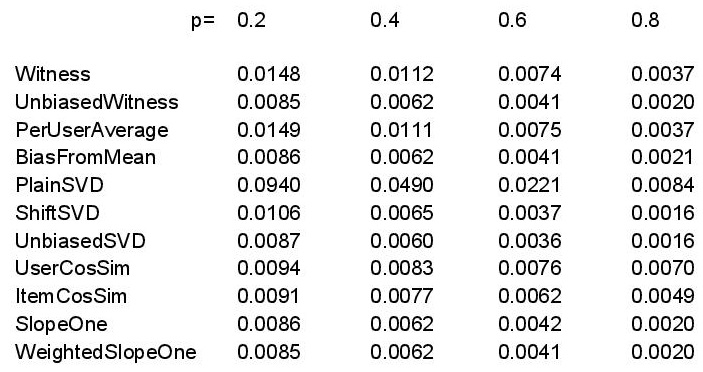
\includegraphics[width=\linewidth]{resultatsPrerapport.jpg}
		\end{figure}
		Sur la matrice du DM, on obtient ce tableau d'erreurs MSE pour différentes valeurs de p :
		
		Eigentaste et quelques autres ne sont pas encore implémentés.
		à venir aussi : une autre mesure d'erreur, et des mesures sur les autres jeux de données.
		
	\subsection{Temps d'exécution}
	
		\begin{figure}[ht!]
			\centering
			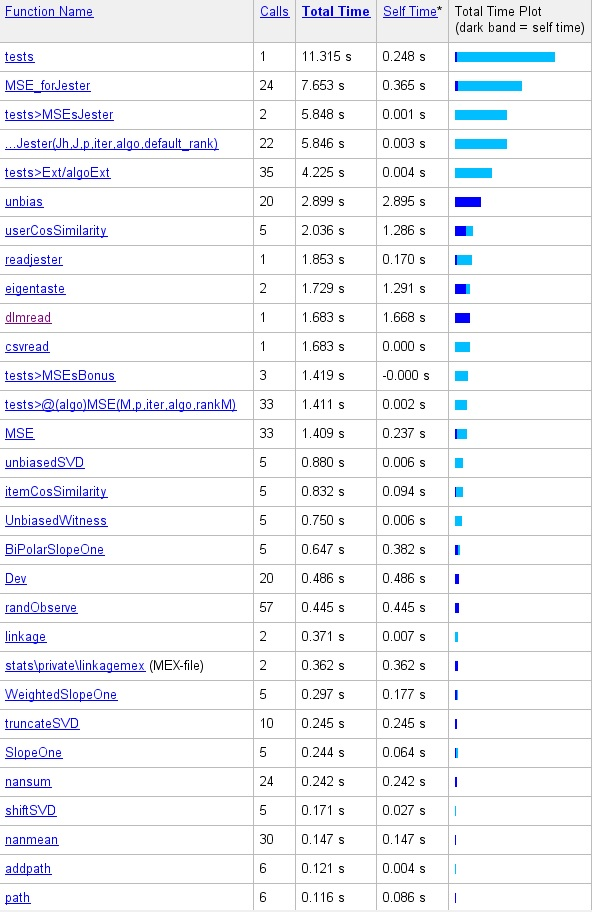
\includegraphics[height=120mm]{times.jpg}
			\caption{Profiling fourni par Matlab}
		\end{figure}
		

		Les algorithmes qui enlèvent et remettent les biais comme dans le cours s'exécutent beaucoup plus lentement : il faut inverser une matrice creuse, et on n'a pas réussi à vectoriser une partie du calcul de l'argmin pour les biais. Il faudra essayer l'expression plus naïve des biais et voir ce qu'on gagne en temps/perd en précision.
		
		Il faut aussi tenir compte du fait que certains algos (Slope One oui, SVD non) calculent des choses "une fois pour toutes", et c'est rapide d'ajouter un utilisateur et/ou de faire une requête.
		
\bibliographystyle{plain}
\bibliography{biblio}

\end{document}